\documentclass[12pt]{article}
\usepackage[utf8]{inputenc}
\usepackage{amsmath}
\usepackage{subcaption}
\usepackage{float}
\usepackage{graphicx}
\usepackage{epstopdf}
\usepackage{color}
\newcommand{\de}[1]{$\langle${{\color{cyan}\slshape{\bfseries DE:} #1}$\rangle$}}
\newcommand{\rz}[1]{$\langle${{\color{magenta}\slshape{\bfseries RZ:} #1}$\rangle$}}

\setlength{\parindent}{4em}
\setlength{\parskip}{1em}
\renewcommand{\baselinestretch}{1.5}

\title{Intensional infect proportion of susceptible}

\begin{document}
\maketitle

\de{There is some rate at which susceptibles are intentionally infected, say $r$, so there is a term $-rS$ in the dimensional SIR equations.  We are expressing the SIR model in dimenionless form, so let $\eta=r/(\gamma+\mu)$ and then we get the following.}

Here is the system we are investigating:
\begin{align}
\frac{\mathrm{d}S}{\mathrm{d}\tau}&=\epsilon -\mathcal{R}_0 SI-\eta S-\epsilon S\\
\frac{\mathrm{d}I}{\mathrm{d}\tau}&=\eta S+\mathcal{R}_0 SI-I\\
\frac{\mathrm{d}R}{\mathrm{d}\tau}&=(1-\epsilon)I-\epsilon R
\end{align}

Here $\gamma$ is mean infectious period, $\mu$ is birth/death rate, $r$ is rate of intensional infection. $\epsilon=\frac{\mu}{\gamma+\mu}$, $\mathcal{R}_0$ is the basic reproduction number.

Since last time we discussed that, it is not very meaningful to divide $I$ into $I_T$ and $I_N$. Thus, I just used I this time to investigate the system's equilibrium, stability and other properties.

First of all, for simplicity reasons, let $L=\frac{r}{\gamma+\mu}$.

Thus, the Endemic equilibrium is the following:

\begin{align}
I &= \frac{-(L+\epsilon-\epsilon\mathcal{R}_0)+\sqrt{(L+\epsilon-\epsilon\mathcal{R}_0)^2+4\mathcal{R}_0\epsilon L}}{2\mathcal{R}_0}\\
S &= \frac{1}{\mathcal{R}_0}-\frac{2L}{\mathcal{R}_0(-(L+\epsilon-\epsilon\mathcal{R}_0)+\sqrt{(L+\epsilon-\epsilon\mathcal{R}_0)^2+4\mathcal{R}_0\epsilon L}+2L)}
\end{align}

Jacobian is the following.
\begin{equation}
\mathcal{J} =
\begin{bmatrix}
    \ -\mathcal{R}_0 I-L-\epsilon       & -\mathcal{R}_0 S \\
    \ L+\mathcal{R}_0 I       & \mathcal{R}_0 S-1 \\
\end{bmatrix}
\end{equation}

Again, for simplicity. Let $G=-(L+\epsilon-\epsilon\mathcal{R}_0)+\sqrt{(L+\epsilon-\epsilon\mathcal{R}_0)^2+4\mathcal{R}_0\epsilon L}$.

So Jacobian at E.E. is:

\begin{equation}
\mathcal{J} =
\begin{bmatrix}
    \ \frac{G}{2}-L-\epsilon       & -1+\frac{2L}{G+2L} \\
    \ L+\frac{G}{2}       & -\frac{2L}{G+2L} \\
\end{bmatrix}
\end{equation}

I then tried to use Wolfram Alpha to compute the eigenvalues for me and I got the following:

\begin{figure}[h!]
  \caption{Eigenvalue computations from Wolfram}
  \centering
  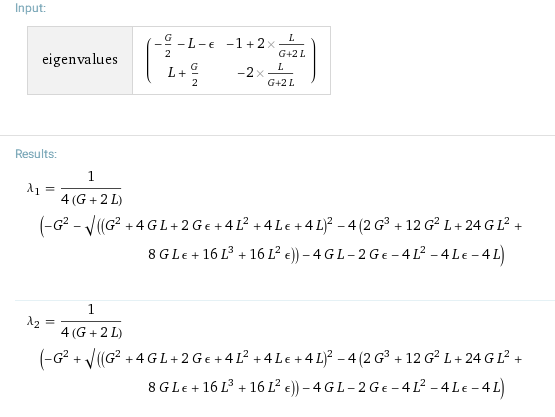
\includegraphics[width=1\textwidth] {Figures/Eigenvalues.png}
\end{figure}

\end{document}